\documentclass{article}
\usepackage{interspeech2005,amssymb,amsmath,epsfig}
\usepackage{amsfonts,amsthm}
\usepackage{float}
\usepackage{xcolor,graphicx}
\usepackage[T1]{fontenc}
\setcounter{page}{1}
%\sloppy         % better line breaks
\ninept
\title{Digit Recognition System Report}  
 \name{Lilian Ye} 
 \address{}
\begin{document}
\maketitle
\begin{abstract}
	In this assignment, a useable digit recognition system has been built. The first part is about an overview of using HTK toolkits for building a recognition system. The key point of the experiment is to decide the best parameters. We have investigated how the three parameters (-t, -s, -p) of HVite influence recognition performance. Also, we carry out experiments to find the optimal number of mixture components.
\end{abstract}

\section{Overview of 	Recognition System}
	This part involves some basic knowledge of using HTK to build a recognition system. You can skip this part if you are familiar with HTK toolkits.   	
\subsection{Data Preparation}
The first stage of any recognizer development project is data preparation. The goal of the system to be built is to recognize digit numbers from zero to nine. So, the recognizer needs to handle digit strings. Examples of typical inputs might be:
$$ \text{three\ \  three\ \  two\ \ six\ \  five\ \  four}$$
HTK provides a grammar definition language for specifying simple task grammars. For this system, a suitable grammar might be:
$$\text{\$digit=eight | five | four | nine | oh | one | seven | six | three | two | zero;}$$
$$\text{(sil < <\$digit> [sp]> sil)} $$
Then convert the grammar to a HTK wordnet lattice using the HParse tool:
$$\text{Harse grammar wordnet}$$
The next step is to build a dictionary. The dictionary provides an association between words used in the task grammar and the acoustic models, which may be composed of sub-word(phonetic, syllabic, etc.) units. As I prefer to use whole-word models in this assignment, the dictionary 'lexicon.dct' has a simple structure. \\[2mm]
\fbox{\begin{minipage}{30mm}
one\  \ \quad one\\
...\\
zero \quad zero\\
sil\quad \quad sil
\end{minipage}}
\\[2mm]
Also, we should create a wordlist 'word.list' which contains all the words in the training materials:\\[2mm]
\fbox{\begin{minipage}{30mm}
one\\
...\\
zero\\
sil
\end{minipage}}
\\[2mm]
Next, we need to tell the recognizer which files correspond to what digits. The transcription files are provided in the form of a Master Label File(MLF) which have been given. Following are the beginning parts of the MLF.\\[2mm]
\fbox{\begin{minipage}{70mm}
\#!MLF!\#\\
"*/MAE\_3A.lab"\\
sil\\
three\\
sil\\
.
\end{minipage}}
\\[2mm]
It is assumed that audio file "MAE\_3A" contains the utterance "three".

\subsection{Feature Extraction}
First, we need to create a configuration file to specify to HTK the nature of the audio data(format, sample rate, etc.) and the feature extraction parameters(type of feature, window length, pre-emphasis, etc.). The template of config file has also been given, which can be changed to suit our needs:\\[2mm]
\fbox{\begin{minipage}{70mm}
TARGETKIND     = MFCC\_E\\
SOURCEFORMAT    = NOHEAD\\
HNET:TRACE     = 1\\
TARGETRATE     = 100000.0\\
SAVECOMPRESSED     = F\\
SAVEWITHCRC     = F\\
...
\end{minipage}}
\\[2mm]
Next, an HTK script file should be created. \\[2mm]
\fbox{\begin{minipage}{70mm}
audio/train/MAE\_3A.08 \  features/train/MAE\_3A.mfc\\
audio/train/MAE\_9A.08 \ features/train/MAE\_9A.mfc\\
...
\end{minipage}}\\[2mm]
One line for each audio file in the training set. The file tells HTK to extract features from each audio file in the first column and save them to the corresponding feature file in the second column. Also, remember to do feature extraction for both devsets and testsets. The HTK command to do the feature extraction is:
$$\text{HCopy -C config -S hcopyfilelist.scp}$$  
\subsection{Training the Models}
First, we should create a prototype HMM ("proto5"), left-to-right configuration with 3 states and 39 dimensional feature vectors as following:
\\[2mm]
\fbox{\begin{minipage}{70mm}
<BeginHMM>\\
<VECSIZE> 39 <MFCC\_E\_D\_A>\\
<NumStates> 5\\
<State> 2\\
  <Mean> 39\\
   0.0 0.0 0.0 ...\\
  <Variance> 39\\
   1.0 1.0 1.0 ...\\
<State> 3\\
...
\end{minipage}}\\[2mm]
Next, create a file "trainlist" that lists all the training feature files, as follows. Don't forget to create "devlist" and "testlist". 
\\[2mm]
\fbox{\begin{minipage}{60mm}
features/train/MAE\_3A.mfc\\
features/train/MAE\_9A.mfc\\
...
\end{minipage}}\\[2mm]
Then, use HCompV to initialize the prototype model with means and variances from the training data. This command creates a master macro file in the 'hmm0' folder which contains copies of the 'proto5' renamed to each of the required models. 
$$\text{HCompV -C config -f 0.01 -m -S trainlist -M models proto5}$$
Then invoke the HERest tool for embedded re-estimation. We can repeat this command a couple of times. 
$$\text{HERest -C config -I MLF -S trainlist -H oldhmm -M newdir mlist}$$
Next, we can fix the 'sp' short pause model by copying the centre state of the 'sil' model to make a new 'sp' model. The 'sp' model looks like this:\\[2mm]
\fbox{\begin{minipage}{60mm}
$\scriptsize{\sim}$h "sp"\\
<BEGINHMM>\\
<NUMSTATES> 3\\
<STATE> 2\\
...
\end{minipage}}\\[2mm]
Then add the extra transitions required and tie the 'sp' state to the centre 'sil' state.
$$\text{HHEd -D -A -T 2 -H newhmm -w hmmfile silfile mlist\_sp}$$
where the silfile contains the following commands:\\[2mm]
\fbox{\begin{minipage}{60mm}
MU 2 {sil.state[2-4].mix}\\
AT 2 4 0.2 {sil.transP}\\
AT 4 2 0.2 {sil.transP}\\
AT 1 3 0.3 {sp.transP}\\
TI silst {sil.state[3],sp.state[2]}
\end{minipage}}\\[2mm]
Then run HERest several more times. 	After it, it's time to increase the number of mixture components from $1$ to $2$. 
$$\text{HHEd -H hmm -M dir incmix.2.hed mlist\_sp}$$
The contents of incmix.2.hed are:\\[2mm]
\fbox{\begin{minipage}{60mm}
MU 2{*.state[2-17].mix}\\
MU 4{sil.state[2-4].mix}\\
MU 4{sp.state[2].mix}
\end{minipage}}\\[2mm]
Then repeat HERest 6 more times to get the updated models. Then increase the number of mixture components from 2 to 3, then retrain, then increase. Repeat this until the final number of mixture components is 18. The acoustic models are now ready.
\subsection{Recognizing Test Data}  
HVite is the Viterbi decoder that performs recognition and HResults can evaluate the performance of the speech recognizer. We ignore some parameters here as we will explain them in next part. 
$$\text{HVite -H hmm -S test.scp -l '*' -i outmlf -w wordnet dict mlist\_sp}$$
$$\text{HResults -I testmlf list\_sp outmlf}$$
Here the outmlf is the mlf file produced by the model, and the testmlf the the correct one. The output is the standard error calculation of replacements, deletions and insertions. 
\section{Experiments and Discussion}
As the datasets are pretty small, so the speed of different parameters varies a little. So we focus on the accuracy for performance evaluation. We use the given dev datasets here. 
\subsection{Parameters for Recognition}
There are a bunch of parameters that control the Viterbi search. And three parameters of HVite play an important role for the results of recognition. 
\begin{itemize}
\item \textbf{Pruning}: (-$t$ $f$) Set $t > 10$ to enable beam searching such that any model whose maximum log probability token falls more than f below the maximum for all models is deactivated. The default value of $t$ is $0.0$ which disables the beam search mechanism. 
\item \textbf{Language model scaling factor}: ($s$ $f$). This factor post-multiplies the language model likelihoods from the word lattices. When the log probabilities for acoustic model and language model are summed, the LM can be weighted. 
\item \textbf{Word insertion probability}: (-$p$ $f$). This parameter controls insertion/deletion ratio. A good rule of thumb is to make number of insertion and deletion errors equal. We optimize this parameter after setting the LM scaling factor. 
\end{itemize}
We first carry out experiments to decide the best parameter for $t$. Figure 1 shows the error rates for different $t$. However, it turns out that setting $t$ to default value to disable the beam search mechanism is the best choice. 
\begin{figure}[H]
\begin{center}
  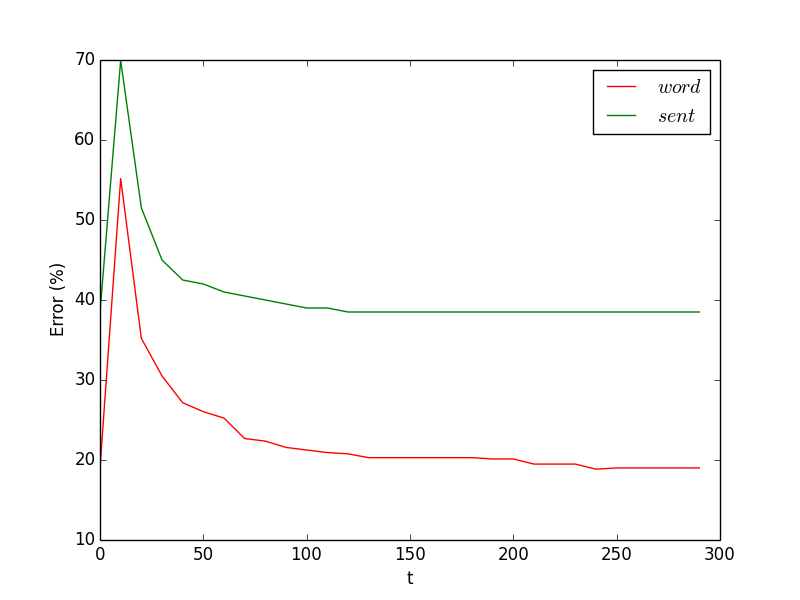
\includegraphics[width=0.52\textwidth]{err_t2.png}
  \caption{Error rate with $t$}\label{err_t}
\end{center}
\end{figure}
Next, we consider the influence of parameter $s$ on the final result. However, it seems that no matter how I change the value of $s$, the error rate keeps the same. So I keep $s$ to its default value. \\
The last important parameter is $p$ and the experiments show that it do have a great influence on the error rate. The word error rate decreases from about $20\%$ to $3\%$ which is a great improvement. The figure 2 shows that the best choice of $p$ is $-100$. 
\begin{figure}
\begin{center}
  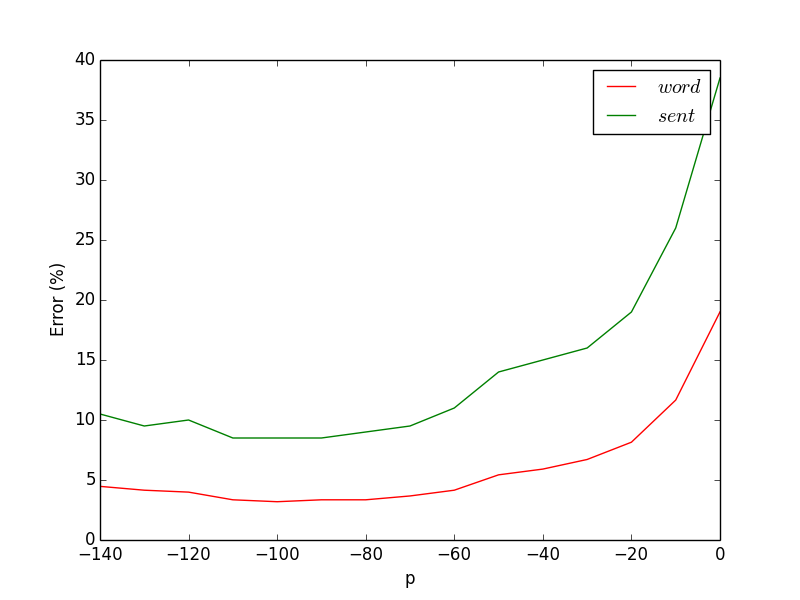
\includegraphics[width=0.52\textwidth]{err_p.png}
  \caption{Error rate with $p$}\label{err_p}
\end{center}
\end{figure}
\subsection{Parameters for Training}
We increase the number of mixture components one by one from $2$ to $18$.  Table 1 shows the process.\\
\begin{table}
\caption{\label{table1} {\it 	Process of Increment}}
\vspace{2mm}
\centerline{
\begin{tabular}{|c|c|c|c|}
\hline
 \# mix & splitting & retraining & final model \\
  \hline
1 &  &hmm11,...,hmm16  & hmm16 \\
2&hmm16->hmm20 & hmm21,...,hmm26 & hmm26 \\
3 & hmm26->hmm30 & hmm31,...,hmm36 & hmm36 \\
... & ... & ... & ...\\
18 & hmm176->hmm180 & hmm181,...,hmm186 & hmm186\\
\hline
\end{tabular}}
\end{table}
After choosing the best parameters for recognition, we then change the number of mixture components to decide the best choice considering the error rate and speed. The error rate decreases from about $9\%$ to $3\%$. Figure 3 shows that setting the number of mixture components to 16 gives the best result. 
\begin{figure}[H]
\begin{center}
  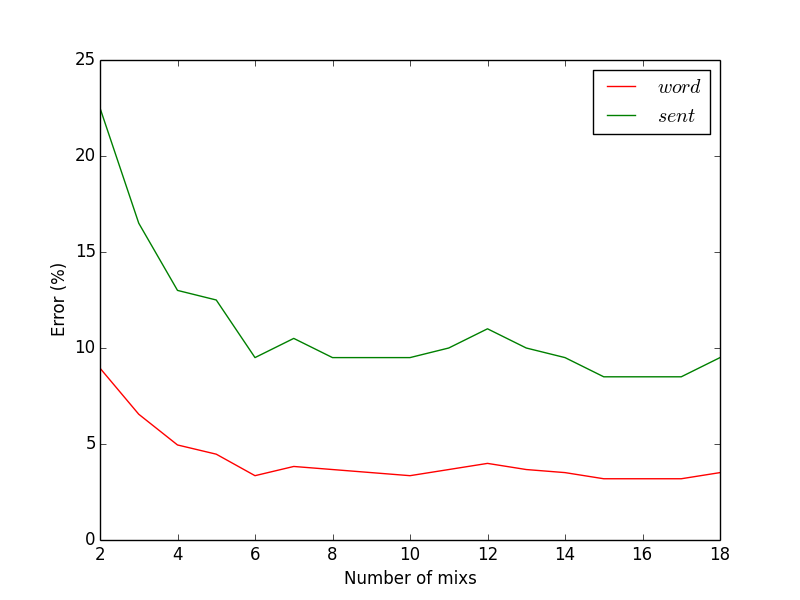
\includegraphics[width=0.52\textwidth]{err_mixs.png}
  \caption{Error rate with number of mixs}\label{err_mixs}
\end{center}
\end{figure}
Next, we want to show why we need retraining after increasing the number of mixture components and what the least times of retraining we need. At first, we retrain 6 times after each increment. Figure 4 shows the result of retraining after increasing the number of mixture components from 2 to 5. Figure 5 shows the result of retraining after increasing the number of mixture components from 6 to 9. It seems that 6 is a little bit too much. At some points, the error rate increases a little after retraining. So we will re-decide the retraining number according to the accuracy. 
\begin{figure}[H]
\begin{center}
  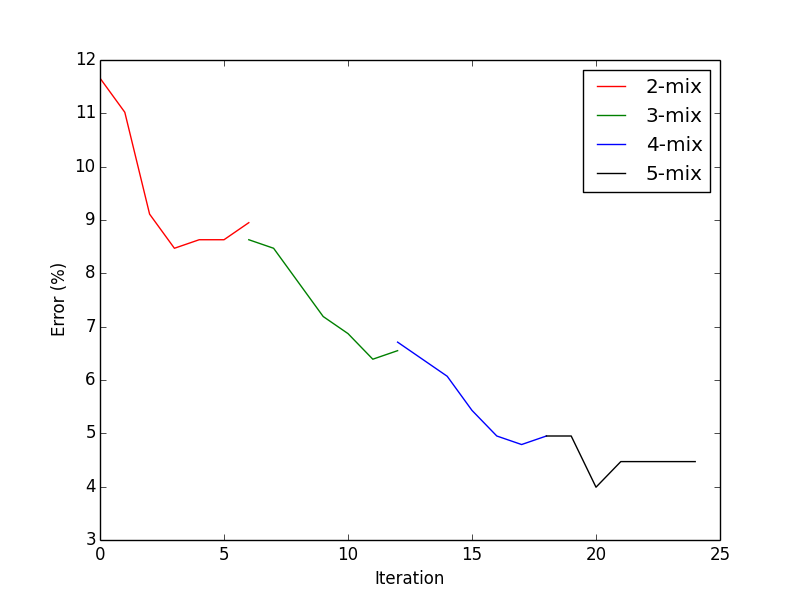
\includegraphics[width=0.52\textwidth]{mix2-mix5.png}
  \caption{Error rate during Iteration 2 to 5}\label{mix2-mix5}
\end{center}
\end{figure}
\begin{figure}[H]
\begin{center}
  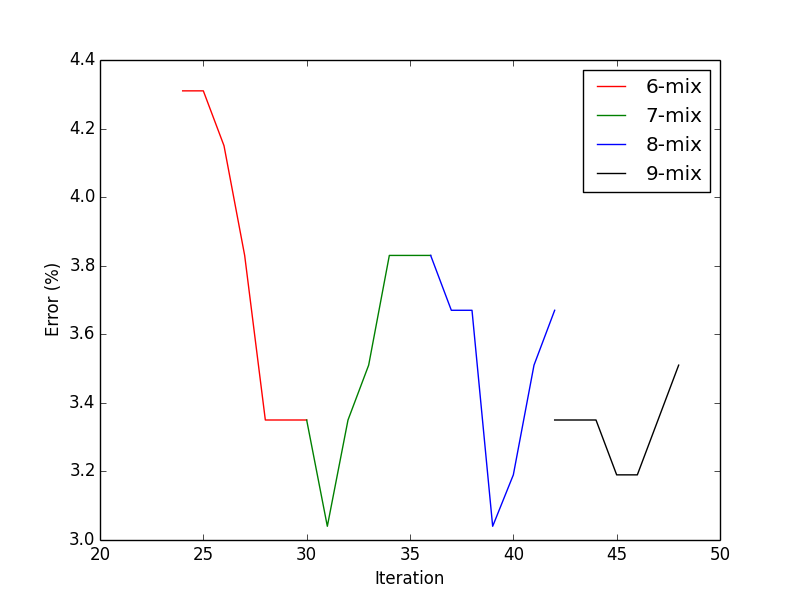
\includegraphics[width=0.52\textwidth]{mix6-mix9.png}
  \caption{Error rate during Iteration 6 to 9}\label{mix6-mix9}
\end{center}
\end{figure}
After decreasing the retraining number from 6 to 5, the best accuracy decreases, but, the best choice of number of mixture components decreases from 16 to 13. Table 2 shows that 6 is still the best choice. \\
\begin{table}
\caption{\label{table1} {\it Experiments of retraining number }}
\vspace{2mm}
\centerline{
\begin{tabular}{|c|c|c|}
\hline
 \# of retrain & word error (\%) & best \# of mixs \\
  \hline
 7 & 3.19 & 11\\
6 & 2.88 & 16\\
5& 3.19 & 13 \\
4 & 3.04 & 7\\
3 & 3.19 & 11\\
\hline
\end{tabular}}
\end{table}
Table 3 shows the best error rate of dev datasets. It's a pretty nice result considering the difficulty of speech recognition. 
\begin{table}
\caption{\label{table1} {\it Best results of devsets }}
\vspace{2mm}
\centerline{
\begin{tabular}{|c c c c c c c|}
\hline
 \# Snt &  Corr & Sub & Del & Ins &Err  & S. Err  \\
 200 & 97.44 &2.08 & 0.48& 0.32&  2.88 & 7.50 \\
\hline
\end{tabular}}
\end{table}

\section{Acknowledgements}
Thanks for Prof. Yu's course, which helps me learn a lot about speech recognition and solve many confusions. Also many thanks for offering the chance of project. Also I am grateful for the teaching assistant Yongbin You, who helped me a lot. 
\end{document}
